\appendix
\chapter*{Chip Gallery}~\label{appendix:chip_gallery}
\markboth{Chip Gallery}{}
\addcontentsline{toc}{chapter}{Chip Gallery}
\renewcommand{\chaptermark}[1]{\markboth{Appendix}{}} 

This chapter showcases a set of chips built on the \mbox{X-HEEP} platform~\cite{x-heep}, listed in chronological order from the earliest to the most recent, highlighting its flexibility in accommodating diverse accelerator architectures, peripheral sets, and application requirements. The direct contributions of the author are focused on the TSMC \SI{65}{\nano\meter} CMOS \mbox{HEEPocrates}~\cite{heepocrates} chip and the TSMC \SI{16}{\nano\meter} CMOS \mbox{HEEPatia} chip, which mark key steps in the platform evolution, from its first silicon implementation to a complex, multi-core, heterogeneous system-on-chip (SoC). The remaining chips demonstrate how research collaborators have extended \mbox{X-HEEP} with custom accelerators or analog front ends to target specific domains such as safety-critical processing, coarse-grained reconfigurable computing, and physiological signal acquisition. Together, these tapeouts span multiple technology nodes and integration strategies, illustrating the role of \mbox{X-HEEP} as a common foundation for heterogeneous computing research.

\clearpage

\begin{center}
\LARGE \bfseries HEEPocrates
\end{center}

\vspace{+1.5em}
\begin{figure}[h]
    \centering
    
\includegraphics[width=0.75\textwidth]{./figures_x-heep/heepocrates.png}
    \caption*{HEEPocrates Layout in TSMC \SI{65}{\nano\meter} LP.}
    \label{fig:heepocrates}
\end{figure}
\vspace{+2em}
\thispagestyle{plain}
HEEPocrates~\cite{heepocrates} is the first silicon implementation of \mbox{X-HEEP} developed by the Embedded Systems Laboratory (ESL) of EPFL. Taped out in November 2022, the SoC features a CV32E20 CPU~\cite{zeroriscy}, \SI{256}{\kibi\byte} of memory organized into eight \SI{32}{\kibi\byte} banks, and a peripheral set comprising a DMA, two SPI interfaces, an I2C interface, GPIOs, a UART, and JTAG. It integrates the OpenEdgeCGRA coarse-grained reconfigurable array (CGRA)~\cite{oe-cgra} and the Blade in-memory computing (IMC) macro~\cite{blade}, with clock generation provided by a frequency-locked loop (FLL) from the PULP platform. Fabricated in TSMC \SI{65}{\nano\meter} LP CMOS technology using low-voltage threshold (LVT) cells, \mbox{HEEPocrates} targets ultra-low-power healthcare applications, which often impose diverse data size, performance, and energy constraints. To address these requirements, it employs fine-grained power domains that allow precise control over component activation. The CPU resides in its own power domain and is typically power-gated during long acquisition phases, waking only upon interrupts generated when the SPI-DMA subsystem completes data transfers.

\clearpage

\begin{center}
\LARGE \bfseries HEEPnosis
\end{center}

\vspace{+1.5em}
\begin{figure}[h]
    \centering
    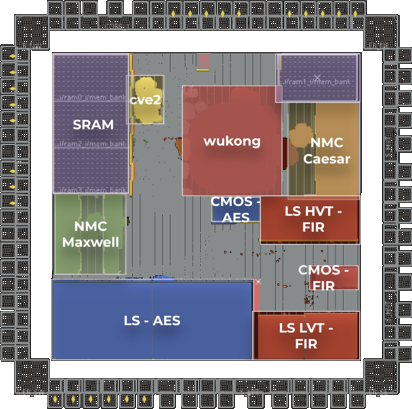
\includegraphics[width=0.7\textwidth]{./figures_x-heep/heepnosis.png}
    \caption*{HEEPnosis Layout in GF \SI{22}{\nano\meter} FDX.}
    \label{fig:heepnosis}
\end{figure}
\vspace{+2em}
\thispagestyle{plain}
HEEPnosis is the second silicon implementation of \mbox{X-HEEP}, developed through a collaboration between the Embedded Systems Laboratory (ESL) and Telecommunication Circuits Laboratory (TCL) of EPFL. Taped out in February 2025, the SoC features a CV32E20 CPU~\cite{zeroriscy} and \SI{128}{\kibi\byte} of memory split into four \SI{32}{\kibi\byte} banks, with two arranged contiguously and two interleaved. Its peripheral set includes two DMA engines, an SPI interface, GPIOs, a UART, and JTAG. The chip integrates the near-memory computing (NMC) macros NM-Caesar~\cite{nmc} and Maxwell~\cite{maxwell}, along with the Wukong~\cite{wukong} accelerator, and incorporates several test IPs implemented using different logic-suppression styles and transistor flavors. Clock generation is provided by a frequency-locked loop (FLL) from the PULP platform. Fabricated in GF \SI{22}{\nano\meter} FDX technology, using a mix of LVT, high-voltage threshold (HVT), and ultra-high-voltage threshold (UHVT) cells, \mbox{HEEPnosis} is primarily intended to validate the functionality and efficiency of full-custom blocks designed with logic suppression, while also assessing the performance and capabilities of the integrated NMC macros.

\clearpage

\begin{center}
\LARGE \bfseries X-TRELA
\end{center}

\vspace{+1.5em}
\begin{figure}[h]
    \centering
    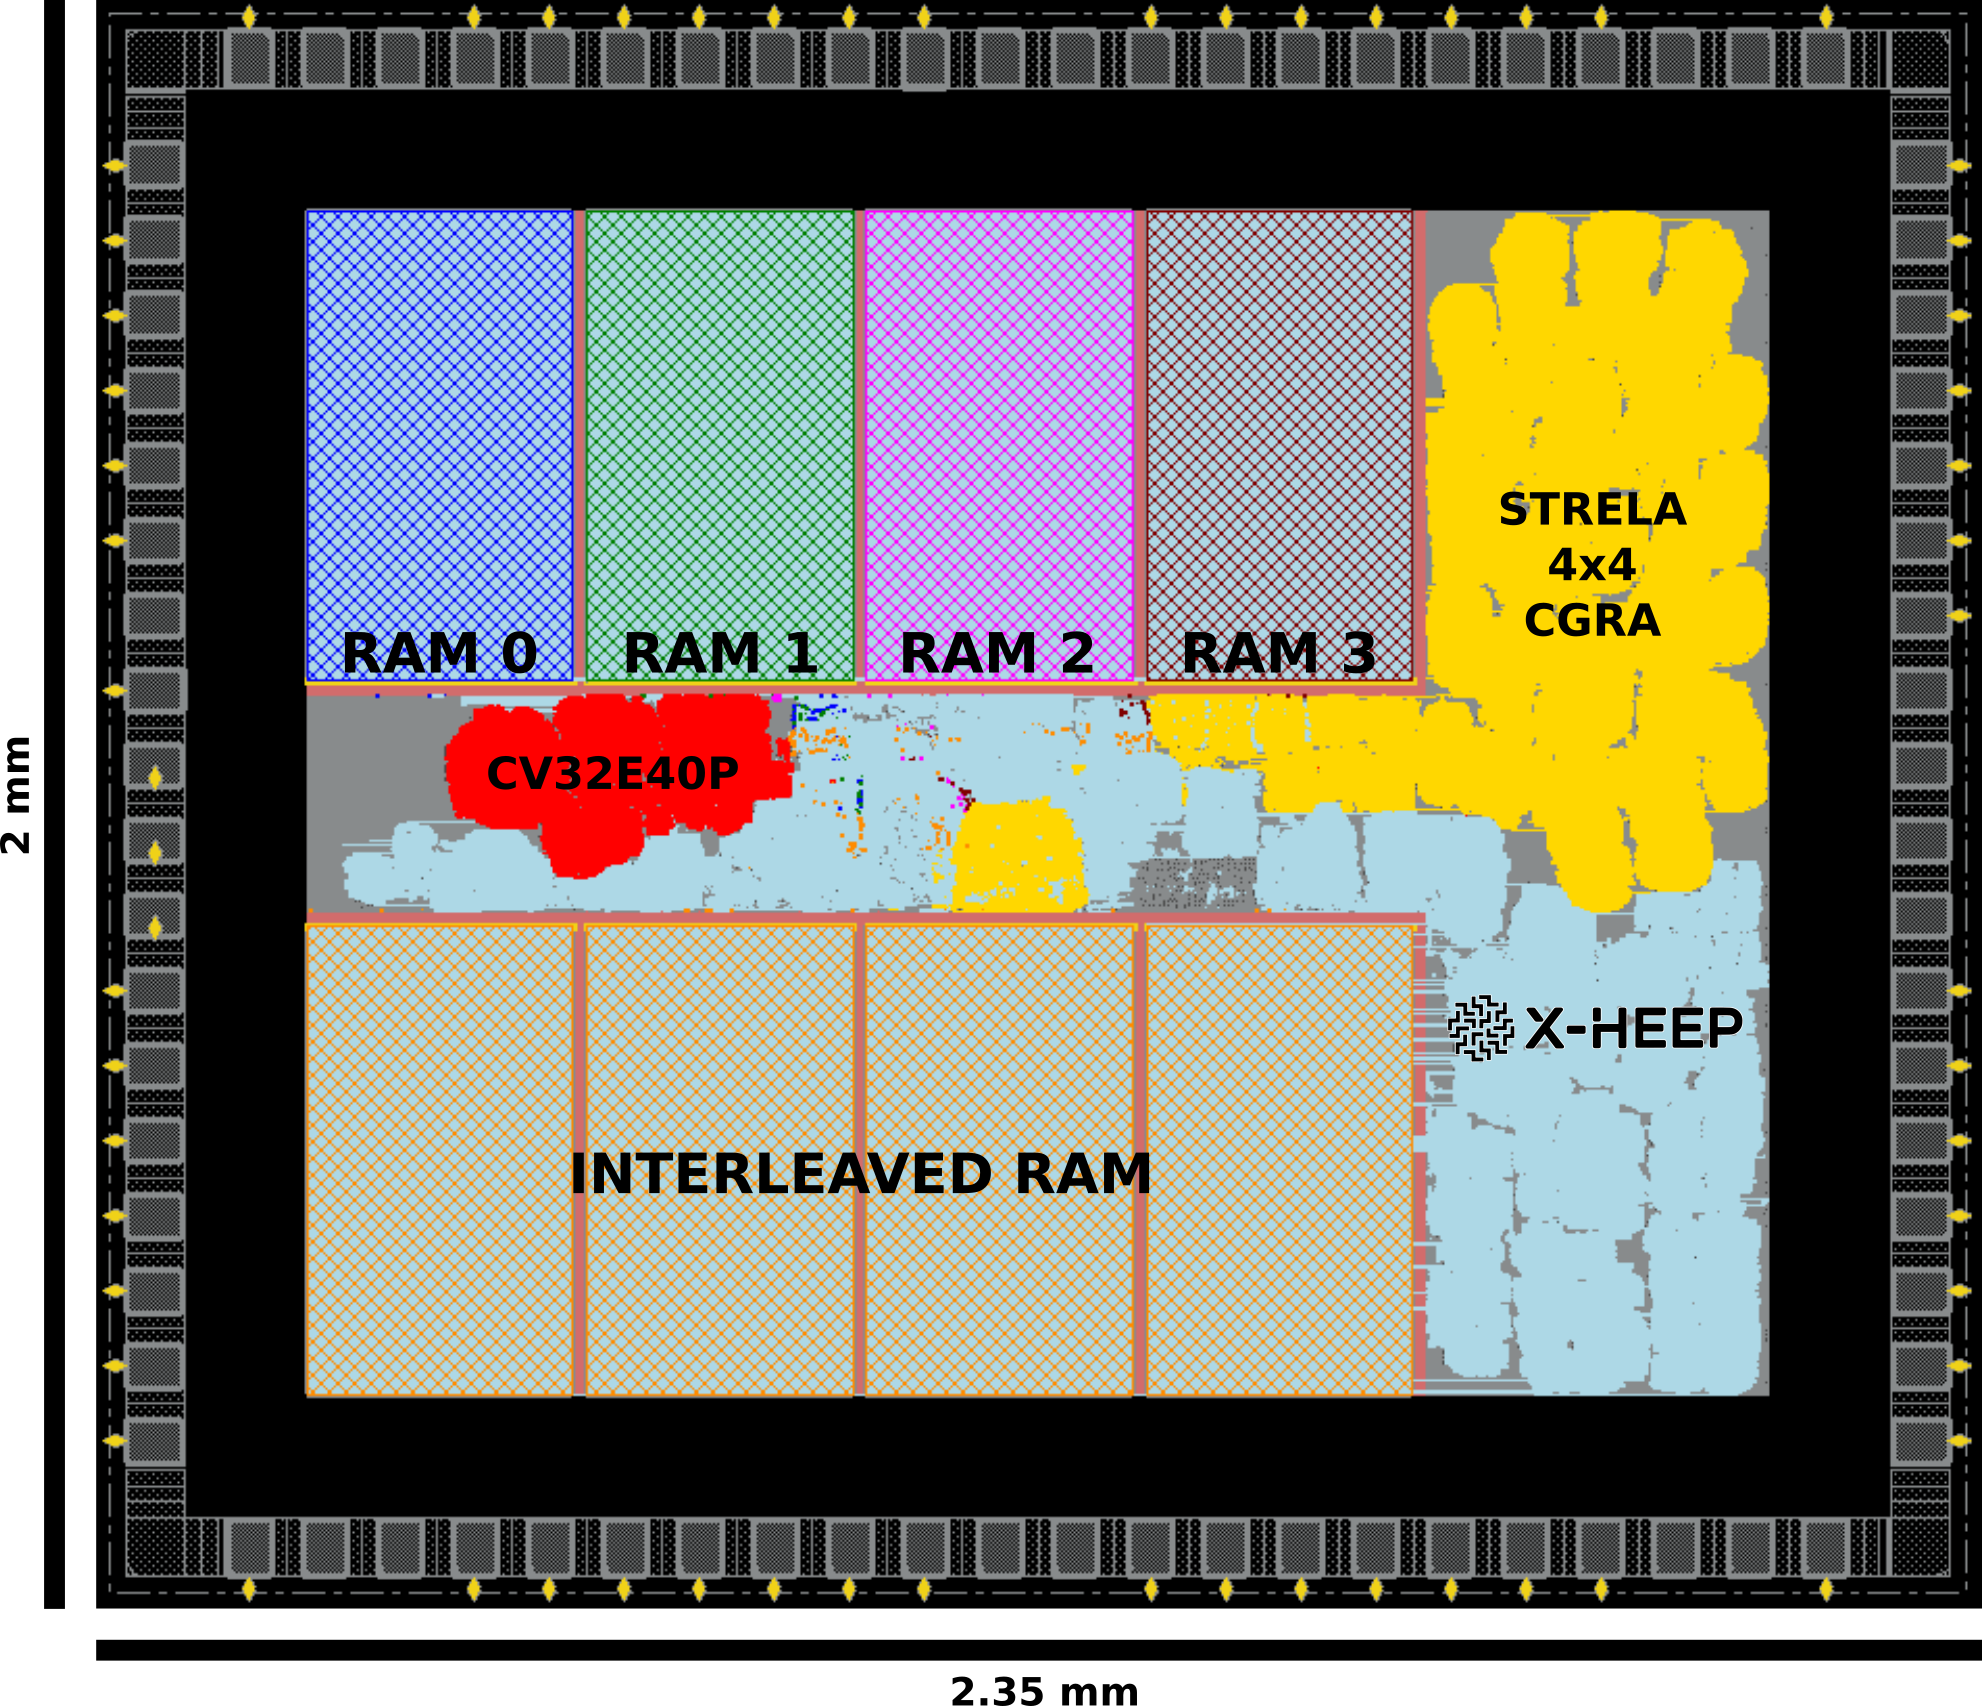
\includegraphics[width=0.75\textwidth]{./figures_x-heep/xtrela.png}
    \caption*{X-TRELA Layout in TSMC \SI{65}{\nano\meter} LP.}
    \label{fig:xstrela}
\end{figure}
\vspace{+2em}
\thispagestyle{plain}
X-TRELA is the third silicon implementation of \mbox{X-HEEP}, developed by the Centro de Electrónica Industrial (CEI) Laboratory of the Universidad Politécnica de Madrid (UPM), Spain. Taped out in February 2025, the SoC features a CV32E40P CPU~\cite{ri5cy}, a fully connected bus, and a total of \SI{256}{\kibi\byte} of memory distributed across four contiguous and four interleaved banks of \SI{32}{\kibi\byte} each. The peripheral set includes a DMA engine, SPI and I2C interfaces, GPIOs, a UART, and JTAG. At its core, X-TRELA integrates the STReaming ELAstic CGRA~\cite{strela}, a 32-bit $4\times4$ array of processing elements designed to efficiently execute dataflow-oriented applications with both data- and control-driven workloads. The design employs low-threshold-voltage cells, slim digital I/Os, CUP bondpads, and ARM-sourced memory macros, and uses a single power domain to simplify the ASIC implementation flow.

\clearpage

\begin{center}
\LARGE \bfseries HEEPidermis
\end{center}

\vspace{+1.5em}
\begin{figure}[h]
    \centering
    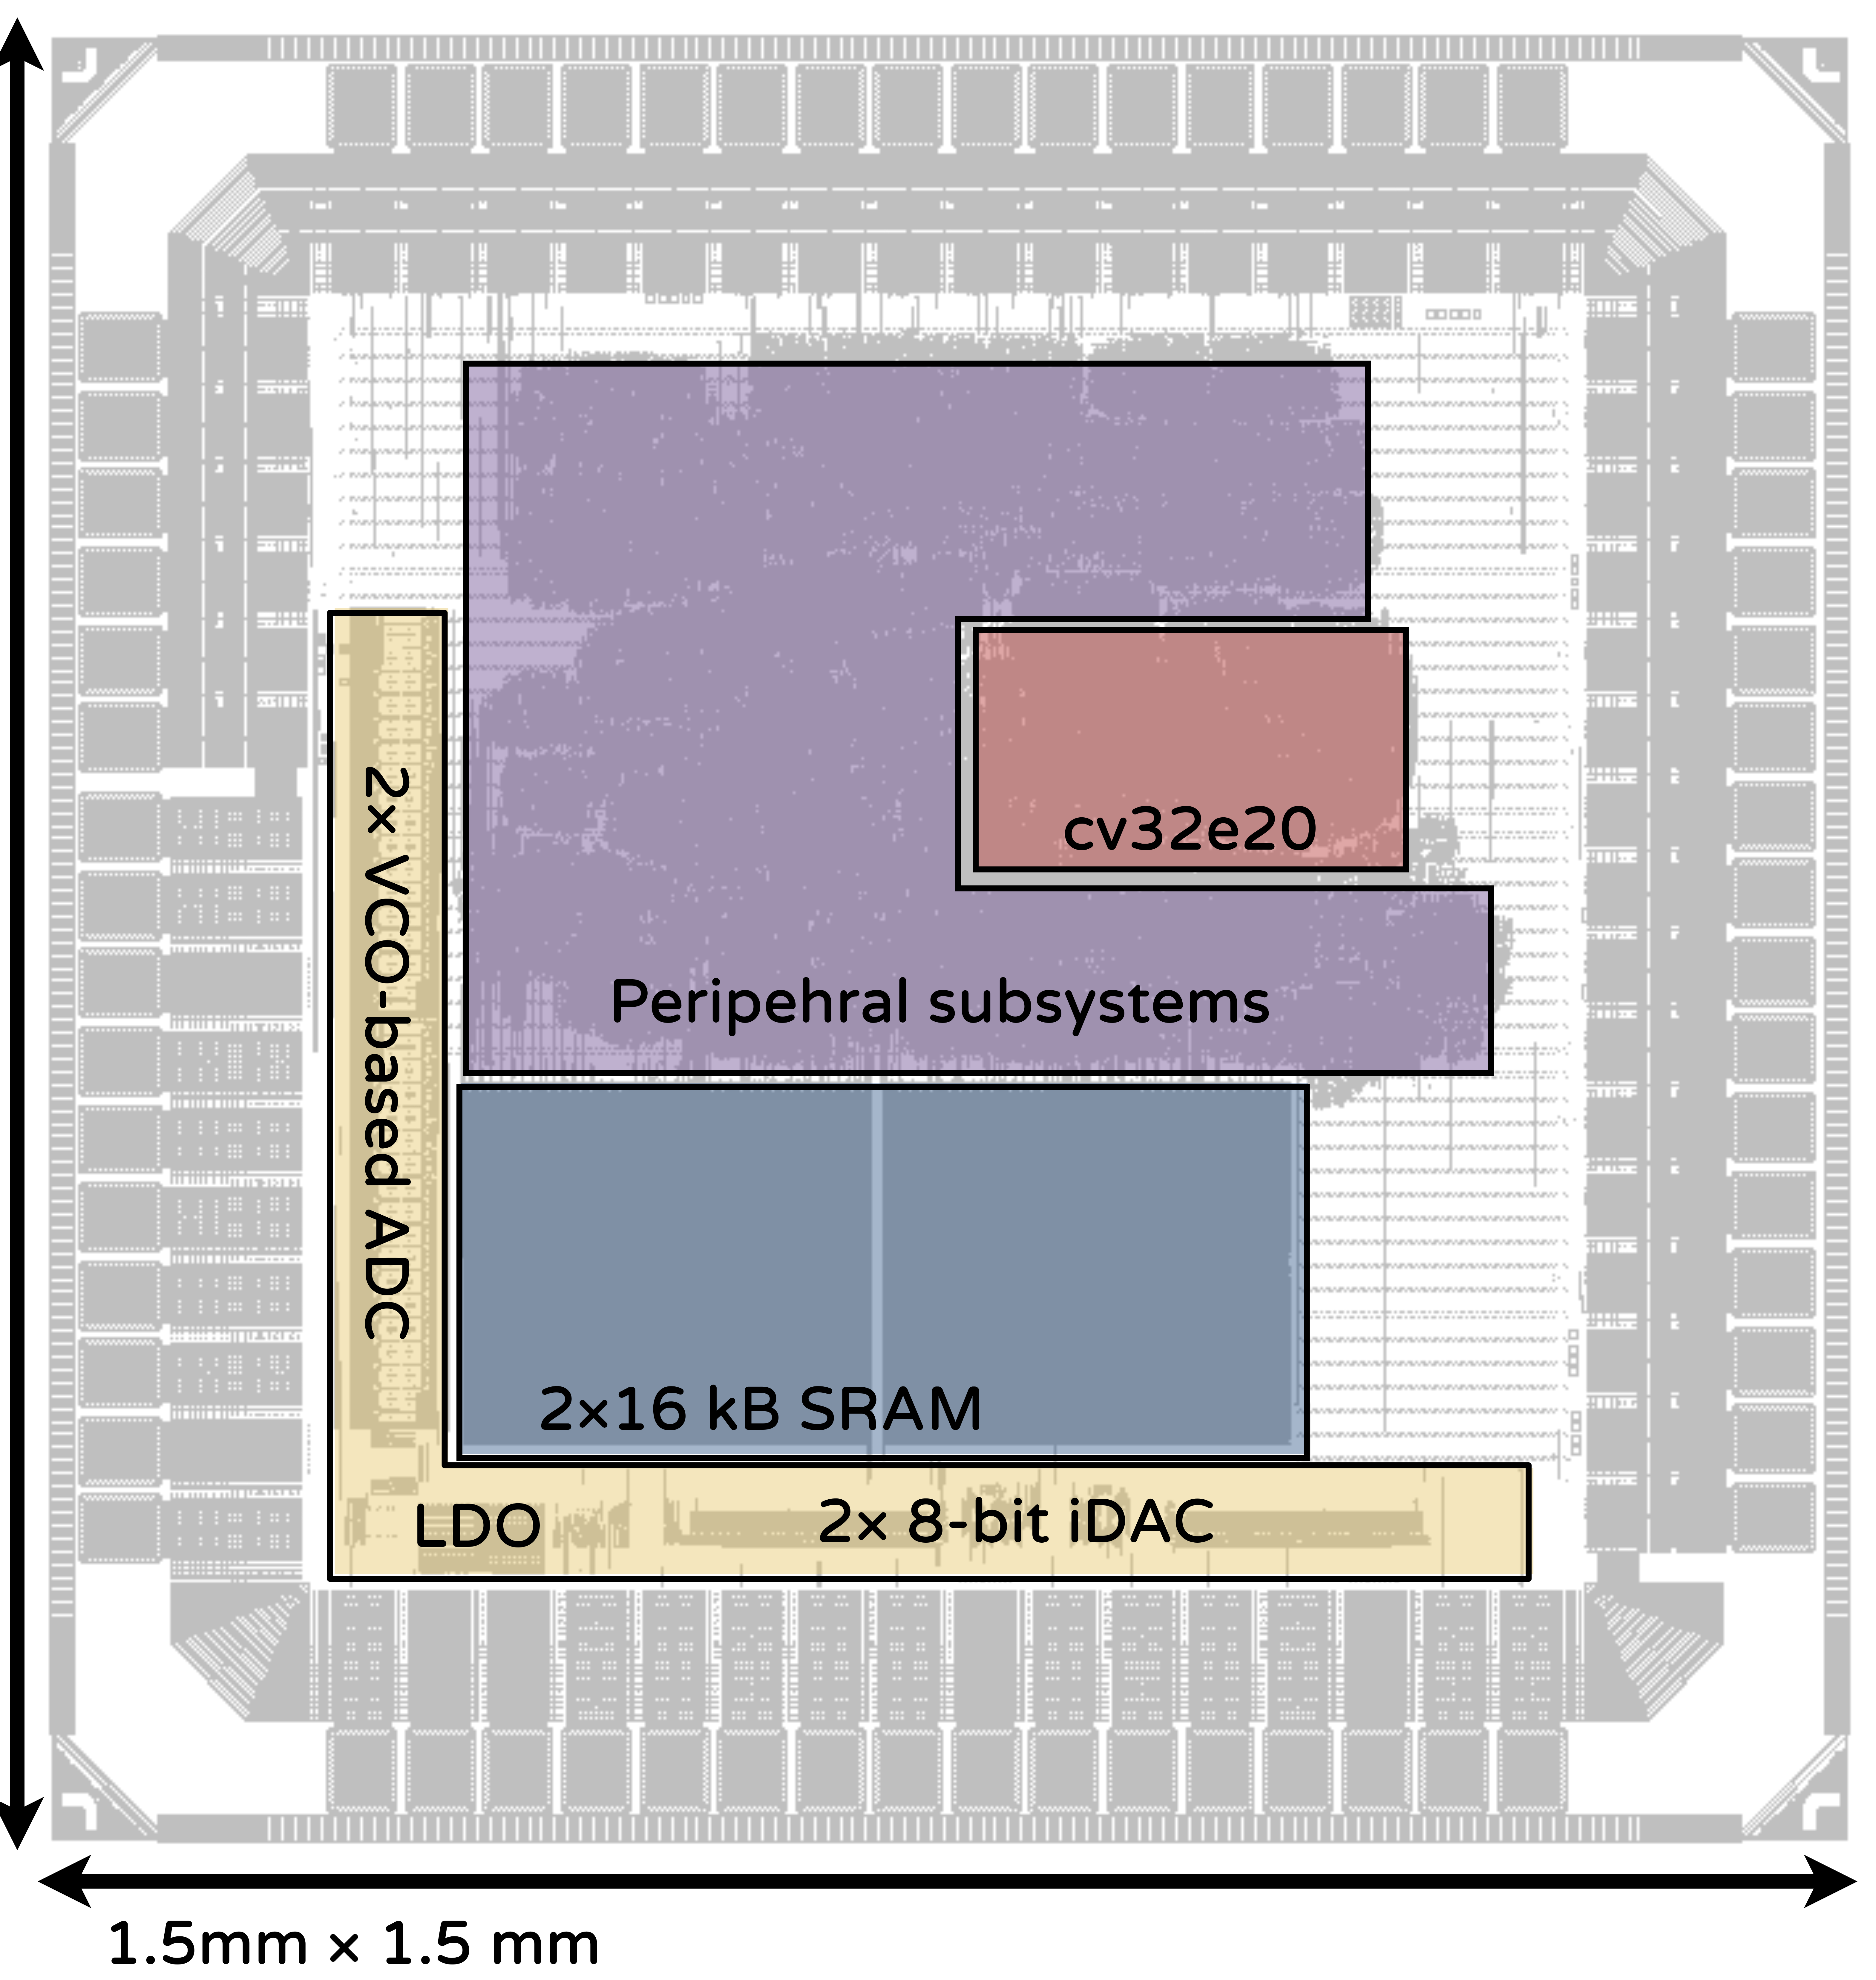
\includegraphics[width=0.7\textwidth]{./figures_x-heep/heepidermis.png}
    \caption*{HEEPidermis Layout in TSMC \SI{65}{\nano\meter} LP.}
    \label{fig:heepidermis}
\end{figure}
\vspace{+2em}
\thispagestyle{plain}
HEEPidermis is the first \mbox{X-HEEP} microcontroller unit extended with an analog front end. It was developed through a collaboration between the Embedded Systems Laboratory (ESL) of EPFL, Universidad Católica del Uruguay (UCU), and Politecnico di Torino. The chip is designed to record galvanic skin response (GSR) signals and integrates two 8-bit current digital-to-analog converters (iDACs) alongside two digitization channels with a VCO-based ADC, which can operate independently or in a pseudo-differential configuration. An integrated DMA engine enables autonomous operation of the iDACs and ADCs, and supports pre-storage data filtering by diverting samples into a Level-Crossing stream accelerator. The chip can function as a high-performance ADC with embedded feature extraction when accessed via its SPI slave interface, and can also control external ADCs for more versatile measurements, either through SPI or via a dedicated $\Delta\Sigma$ input supporting decimation.

\clearpage

\begin{center}
\LARGE \bfseries X-EROS
\end{center}

\vspace{+1.5em}
\begin{figure}[h]
    \centering
    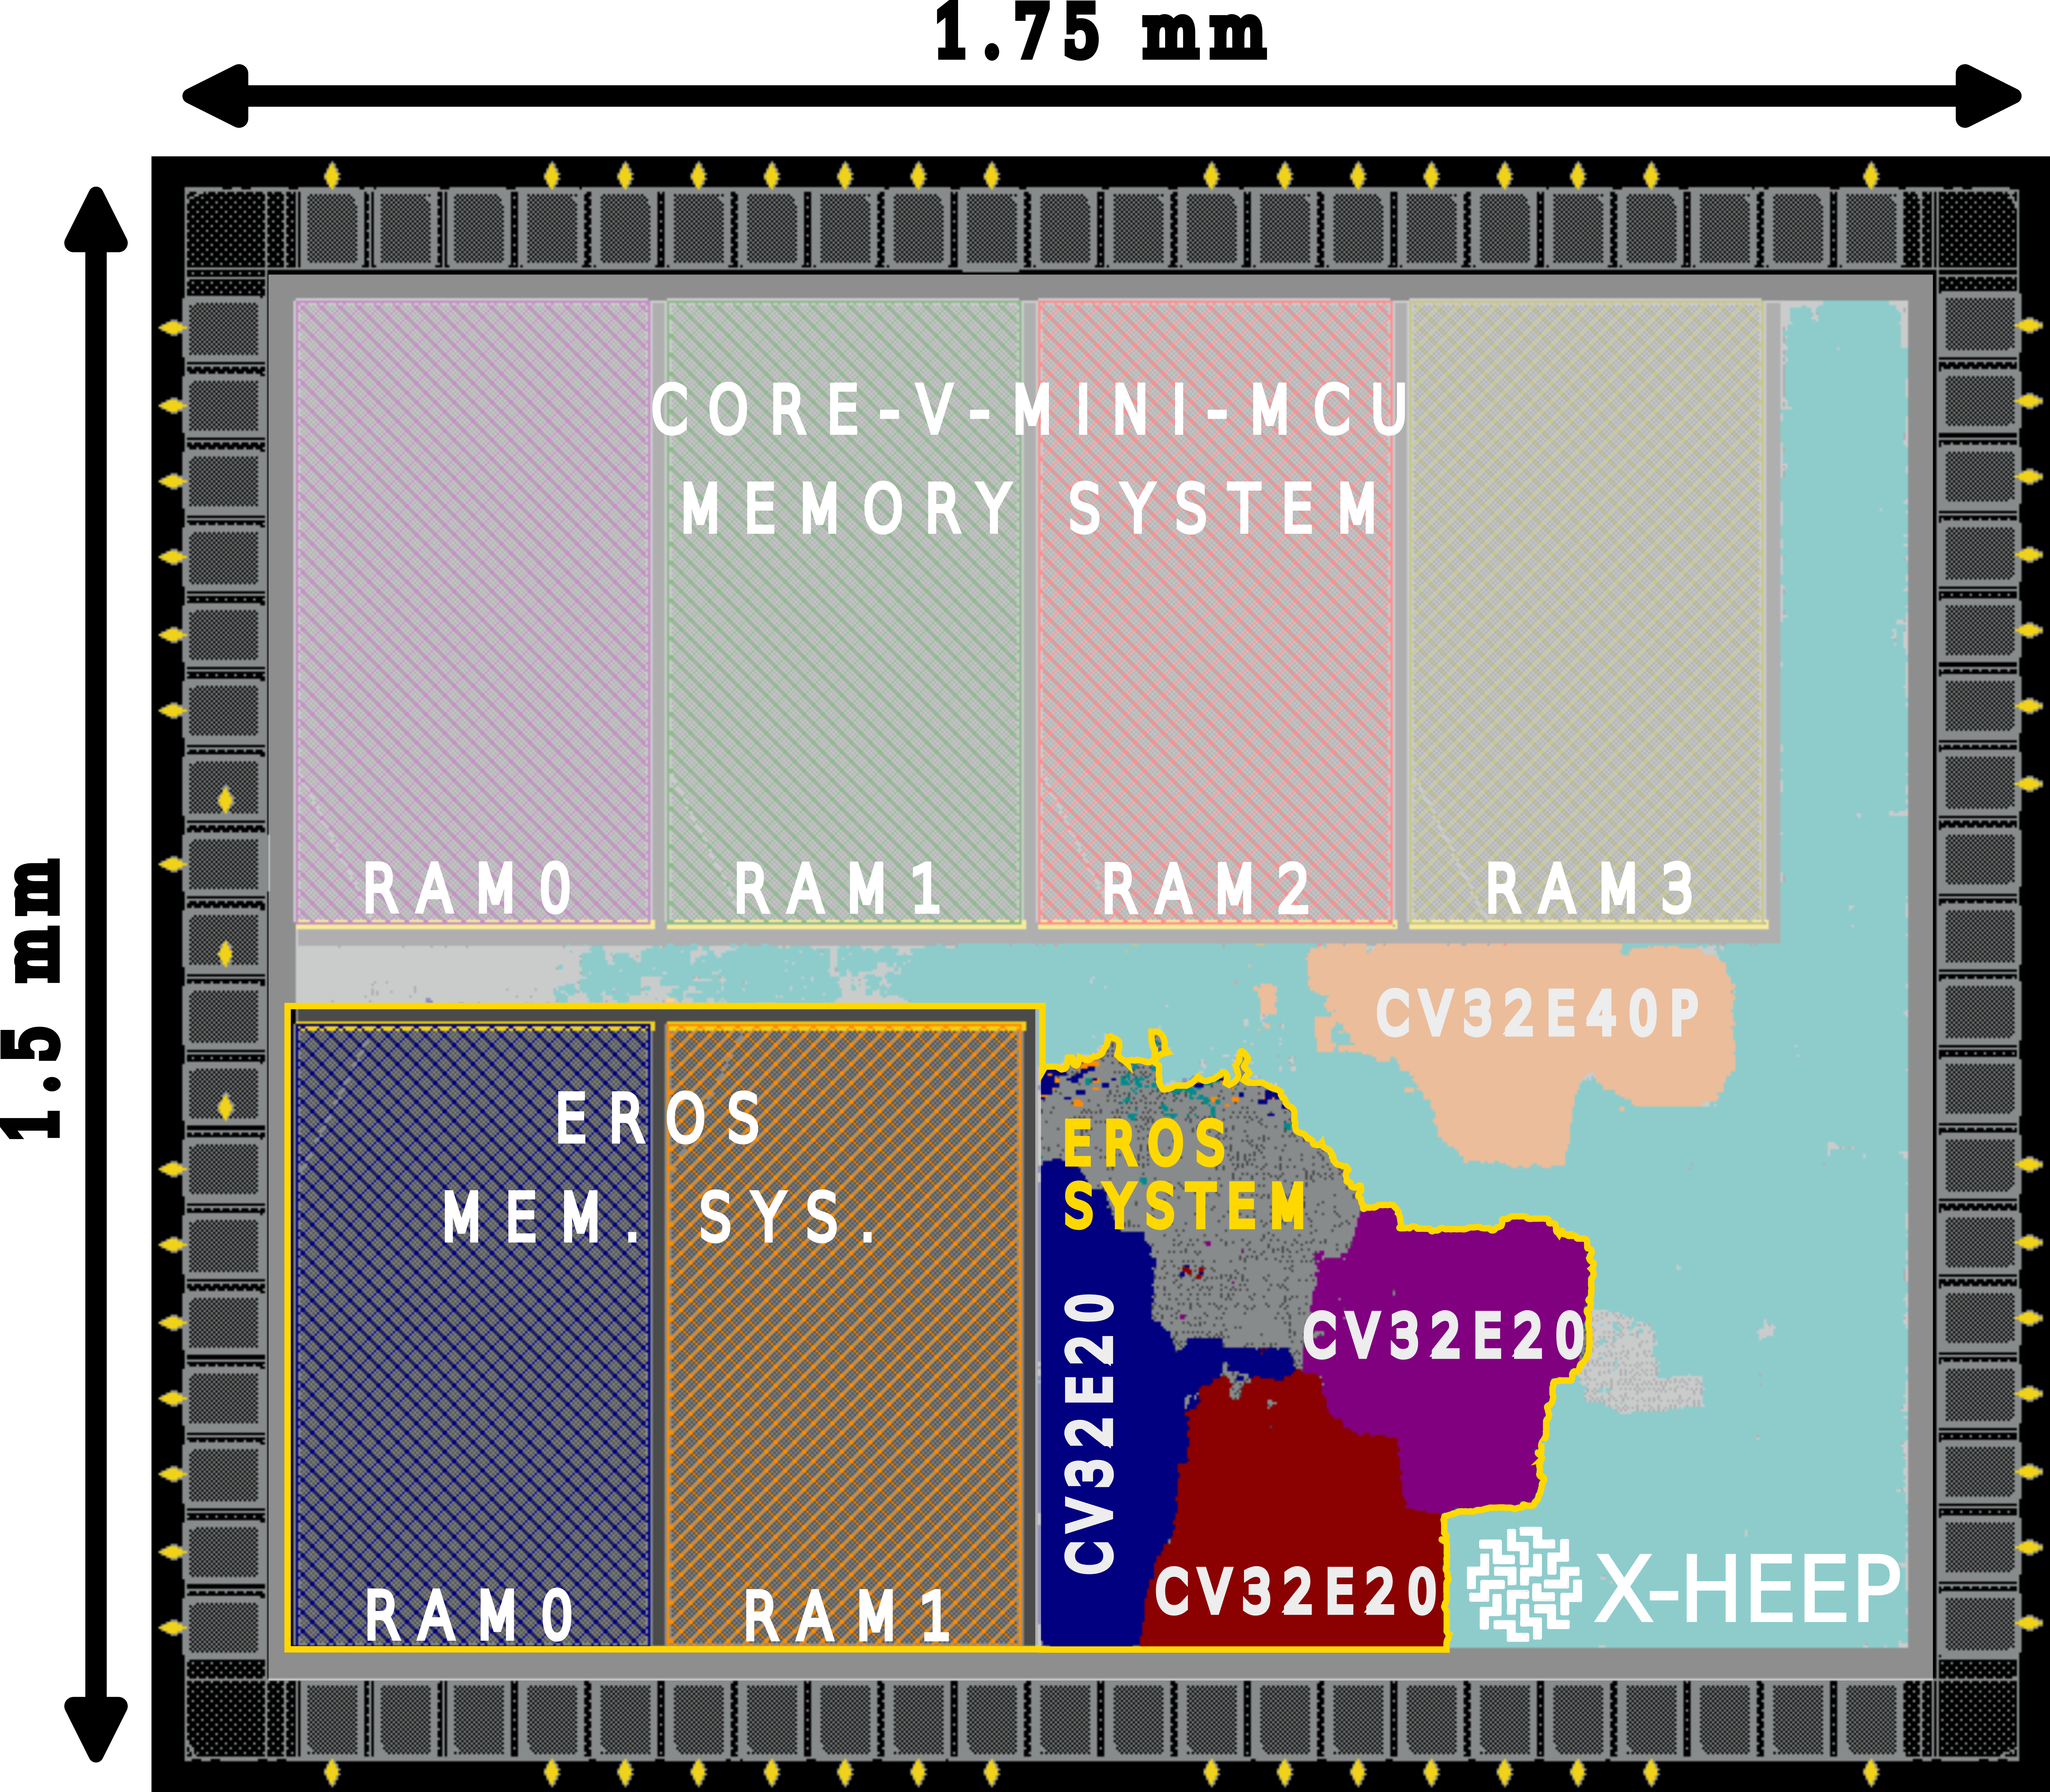
\includegraphics[width=0.75\textwidth]{./figures_x-heep/xeros.png}
    \caption*{X-EROS Layout in TSMC \SI{65}{\nano\meter} LP.}
    \label{fig:xeros}
\end{figure}
\vspace{+2em}
\thispagestyle{plain}
Taped out in June~2025, \mbox{X-EROS} is an \mbox{X-HEEP}-based SoC developed by the Centro de Electrónica Industrial (CEI) Laboratory at the Universidad Politécnica de Madrid (UPM), Spain. Its configuration features a CV32E40P RISC-V CPU~\cite{ri5cy}, an fully connected bus, and four contiguous \SI{128}{\kibi\byte} banks, each composed of \SI{32}{\kibi\byte} sub-banks. The peripheral set includes a DMA controller, SPI and I\textsuperscript{2}C interfaces, GPIOs, a UART, and JTAG. At the core of the design is the Extensible Reliable Offloading Solution (EROS)~\cite{eros}, a safety-critical accelerator island comprising three CV32E20 CPUs~\cite{zeroriscy} capable of operating in both safety and non-safety modes, paired with dedicated \SI{32}{\kibi\byte} instruction and data memory banks. This subsystem is intended for mixed-criticality applications, enabling reliable offloading of safety-sensitive workloads. Implemented using low-threshold-voltage cells, slim digital I/Os, CUP bondpads, and ARM-sourced memory macros, \mbox{X-EROS} employs a single power domain to simplify the ASIC flow and represents the second tapeout by the CEI-UPM group.

\clearpage

\begin{center}
\LARGE \bfseries HEEPatia
\end{center}

\vspace{+1.5em}
\begin{figure}[h]
    \centering
    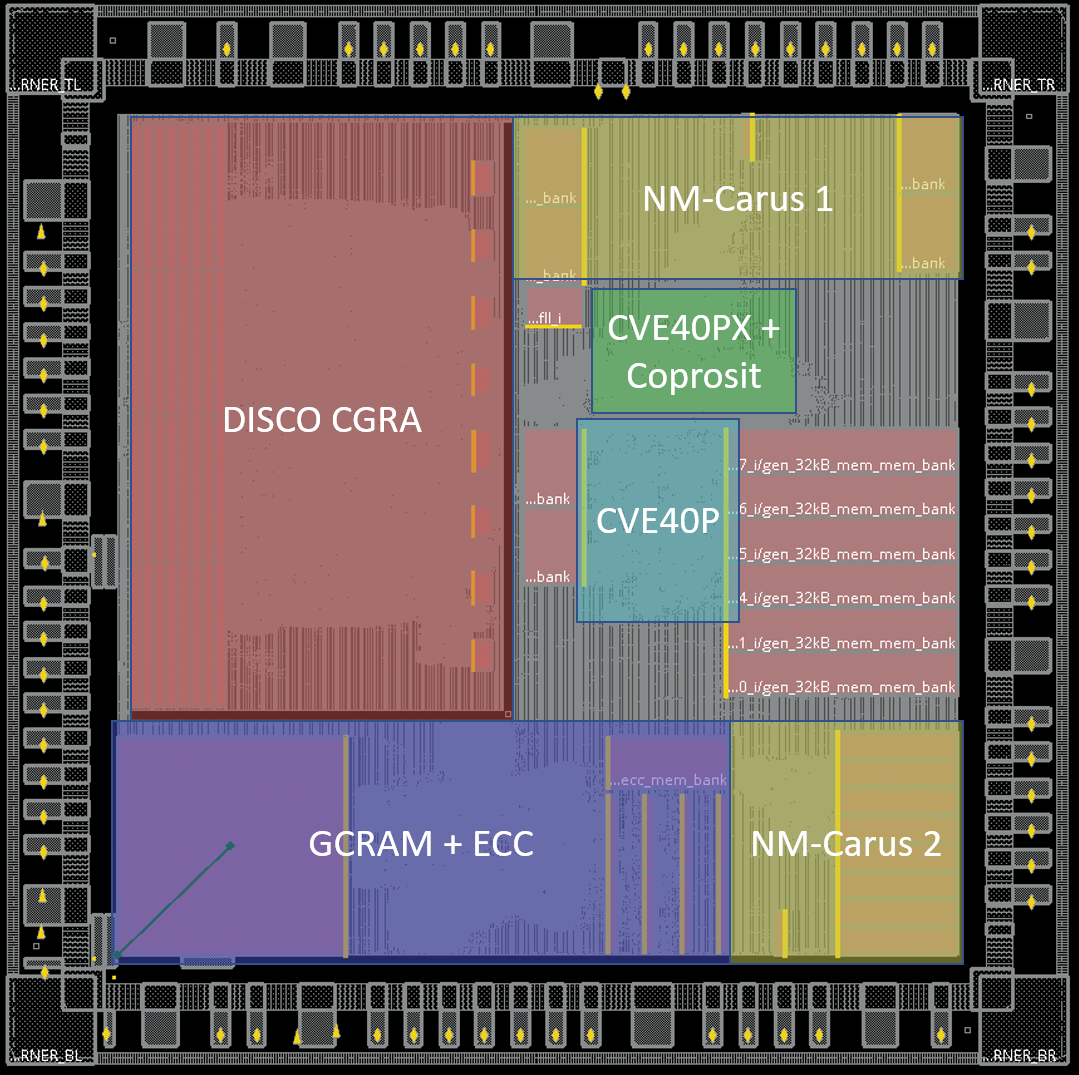
\includegraphics[width=0.7\textwidth]{./figures_x-heep/heepatia.png}
    \caption*{HEEPatia Layout in TSMC \SI{16}{\nano\meter} LP.}
    \label{fig:heepatia}
\end{figure}
\vspace{+2em}
\thispagestyle{plain}
Taped out in July~2025, \mbox{HEEPatia} is the first silicon implementation of the \mbox{X-HEEP} platform in \SI{16}{\nano\meter} TSMC technology, developed through a collaboration between the Embedded Systems Laboratory (ESL) of EPFL, Telecommunication Circuits Laboratory (TCL) of EPFL, and Politecnico di Torino. It adopts a dual-core configuration with the CV32E40P and CV32E40PX RISC-V CPUs~\cite{ri5cy}, the latter extended by the Coprosit coprocessing unit for posit arithmetic~\cite{percival}. The system integrates \SI{608}{\kibi\byte} of on-chip memory, comprising \SI{352}{\kibi\byte} of SRAM and \SI{256}{\kibi\byte} of gain-cell RAM. To accelerate edge-AI workloads, \mbox{HEEPatia} incorporates two NMC NM-Carus accelerators~\cite{nmc}, a DISCO CGRA accelerator~\cite{vwr2a}, and the Coprosit coprocessor~\cite{percival}. Implemented with a combination of low- and standard-threshold cells, the chip is intended as a research platform for evaluating performance, power, and area trade-offs across diverse hardware IPs and for executing edge applications.
